% !BIB program = biber 
\documentclass{article}

%% Encoding
\usepackage[T1]{fontenc}
\usepackage[utf8]{inputenc}

%% Fonts
% Math fonts (fourier) with utopia (erewhon) text fonts
\usepackage{fourier, erewhon}

%% Setup
% This package contains logos
\usepackage[autoload]{adn}
\setlogos[
\textbf{MO433 --- Intro. to Unsupervised Machine Learning}\\%[5pt]
\uppercase{Instituto de Computação --- UNICAMP}\\%[-7pt]
]%
{IC3D}%
{UNICAMP}

%% Transform section references
\makeatletter
\renewcommand*{\p@section}{\S\,}
\renewcommand*{\p@subsection}{\S\,}
\makeatother

%% Shorthands
\usepackage{xspace}
\makeatletter
\DeclareRobustCommand\onedot{\futurelet\@let@token\@onedot}
\def\@onedot{\ifx\@let@token.\else.\null\fi\xspace}

\def\eg{e.g\onedot} \def\Eg{E.g\onedot}
\def\ie{i.e\onedot} \def\Ie{I.e\onedot}
\def\cf{cf\onedot} \def\Cf{Cf\onedot}
\def\etc{etc\onedot} \def\vs{vs\onedot}
\def\wrt{w.r.t\onedot} \def\dof{d.o.f\onedot}
\def\etal{et al\onedot}
\def\idd{i.d.d\onedot}
\makeatother

%%%
% Other packages start here (see the examples below)
%%
\usepackage{float}
\usepackage{caption}
\usepackage{subcaption}
\newcommand\myrowlabel[1]{%
  \rotatebox[origin=c]{90}{#1}%
}
\usepackage{grffile}


%% Figues
% \usepackage[draft]{graphicx}
\usepackage{graphicx}
\graphicspath{{./images/}{../output/}{../input/results/}}

%% References
% Use this section to embed your bibliography
% Instead of having a separate file, just place the bibtex entries here
\usepackage{filecontents}% create files
\begin{filecontents}{\jobname.bib}
  @article{zhang2018,
    author={Jing Zhang and Tong Zhang and Yuchao Dai and Mehrtash Harandi and Richard I. Hartley},
    title={Deep Unsupervised Saliency Detection: {A} Multiple Noisy Labeling Perspective},
    journal={CoRR},
    volume={abs/1803.10910},
    year={2018},
    url={http://arxiv.org/abs/1803.10910},
    archivePrefix={arXiv},
    eprint={1803.10910}
  }
  @article{symonyan2014,
    author={Karen Simonyan and Andrea Vedaldi and Andrew Zisserman},
    title={Deep Inside Convolutional Networks: Visualising Image Classification Models and Saliency Maps},
    journal={CoRR},
    volume={abs/1312.6034},
    year={2014},
    url={https://arxiv.org/pdf/1312.6034.pdf},
    archivePrefix={arXiv},
    eprint={1312.6034}
  }
  @article{zhang2014,
    author={Ali Borji and Ming{-}Ming Cheng and Huaizu Jiang and Jia Li},
    title={Salient Object Detection: {A} Survey},
    journal={CoRR},
    volume={abs/1411.5878},
    year={2014},
    url={http://arxiv.org/abs/1411.5878},
    archivePrefix={arXiv},
    eprint={1411.5878},
  }
  @inproceedings{zhang2017,
    author={D. {Zhang} and J. {Han} and Y. {Zhang}},
    booktitle={2017 IEEE International Conference on Computer Vision (ICCV)}, 
    title={Supervision by Fusion: Towards Unsupervised Learning of Deep Salient Object Detector}, 
    year={2017},
    volume={},
    number={},
    pages={4068-4076}
    }
  @article{wang2017,
    author="Wang, Jingdong and Jiang, Huaizu and Yuan, Zejian and Cheng, Ming-Ming and Hu, Xiaowei and Zheng, Nanning",
    title="Salient Object Detection: A Discriminative Regional Feature Integration Approach",
    journal="International Journal of Computer Vision",
    year="2017",
    volume="123",
    number="2",
    pages="251--268",
    issn="1573-1405",
    doi="10.1007/s11263-016-0977-3"
  }
  @article{Borji2019,
    doi = {10.1007/s41095-019-0149-9},
    file = {:home/marcosf/.local/share/data/Mendeley Ltd./Mendeley Desktop/Downloaded/Borji et al. - 2019 - Computational Visual Media Salient object detection A survey.pdf:pdf},
    isbn = {4109501901499},
    keywords = {regions of interest,saliency,salient object detection,visual attention},
    number = {2},
    pages = {117--150},
    title = {{Computational Visual Media Salient object detection: A survey}},
    url = {https://doi.org/10.1007/s41095-019-0149-9},
    volume = {5},
    year = {2019}
  }
  @INPROCEEDINGS{MBD,  
    author={J. {Zhang} and S. {Sclaroff} and Z. {Lin} and X. {Shen} and B. {Price} and R. {Mech}},  
    booktitle={2015 IEEE International Conference on Computer Vision (ICCV)},   title={Minimum Barrier Salient Object Detection at 80 FPS},   
    year={2015},  
    volume={},  
    number={},  
    pages={1404-1412},
  }
  @INPROCEEDINGS{FT,  
    author={R. {Achanta} and S. {Hemami} and F. {Estrada} and S. {Susstrunk}},  booktitle={2009 IEEE Conference on Computer Vision and Pattern Recognition},   title={Frequency-tuned salient region detection},   
    year={2009},  
    volume={},  
    number={},  
    pages={1597-1604},
  }
  @INPROCEEDINGS{RBD,  
    author={W. {Zhu} and S. {Liang} and Y. {Wei} and J. {Sun}},  
    booktitle={2014 IEEE Conference on Computer Vision and Pattern Recognition},   
    title={Saliency Optimization from Robust Background Detection}, 
    year={2014}, 
    volume={},  
    number={},  
    pages={2814-2821},
  }
  @article{HCRC,
    author = {Cheng, Ming-Ming and Mitra, N and Huang, X and Torr, Philip and Hu, Shi-Min},
    year = {2011},
    month = {10},
    pages = {},
    title = {Salient Object Detection and Segmentation},
    volume = {37},
    journal = {IEEE Transactions on Pattern Analysis and Machine Intelligence},
    doi = {10.1109/TPAMI.2014.2345401},
  }
  @article{Deeplab,
    author    = {Liang{-}Chieh Chen and
                George Papandreou and
                Iasonas Kokkinos and
                Kevin Murphy and
                Alan L. Yuille},
    title     = {DeepLab: Semantic Image Segmentation with Deep Convolutional Nets,
                Atrous Convolution, and Fully Connected CRFs},
    journal   = {CoRR},
    volume    = {abs/1606.00915},
    year      = {2016},
    url       = {http://arxiv.org/abs/1606.00915},
    archivePrefix = {arXiv},
    eprint    = {1606.00915},
    timestamp = {Mon, 13 Aug 2018 16:46:13 +0200},
    biburl    = {https://dblp.org/rec/journals/corr/ChenPK0Y16.bib},
    bibsource = {dblp computer science bibliography, https://dblp.org}
  }
  @article{ResNet101,
    author    = {Kaiming He and
                Xiangyu Zhang and
                Shaoqing Ren and
                Jian Sun},
    title     = {Deep Residual Learning for Image Recognition},
    journal   = {CoRR},
    volume    = {abs/1512.03385},
    year      = {2015},
    url       = {http://arxiv.org/abs/1512.03385},
    archivePrefix = {arXiv},
    eprint    = {1512.03385},
    timestamp = {Wed, 17 Apr 2019 17:23:45 +0200},
    biburl    = {https://dblp.org/rec/journals/corr/HeZRS15.bib},
    bibsource = {dblp computer science bibliography, https://dblp.org}
  }
  @incollection{Amit2017,
    doi = {10.1007/978-3-319-66179-7_68},
    url = {https://doi.org/10.1007/978-3-319-66179-7_68},
    year = {2017},
    publisher = {Springer International Publishing},
    pages = {594--602},
    author = {Guy Amit and Omer Hadad and Sharon Alpert and Tal Tlusty and Yaniv Gur and Rami Ben-Ari and Sharbell Hashoul},
    title = {Hybrid Mass Detection in Breast {MRI} Combining Unsupervised Saliency Analysis and Deep Learning},
    booktitle = {Medical Image Computing and Computer Assisted Intervention - {MICCAI} 2017}
  }
  @INPROCEEDINGS{Zhang2011,
    author={Y. {Zhang} and J. {Shen} and M. {Rotea} and N. {Gans}},
    booktitle={2011 IEEE/RSJ International Conference on Intelligent Robots and Systems}, 
    title={Robots looking for interesting things: Extremum seeking control on saliency maps}, 
    year={2011},
    volume={},
    number={},
    pages={1180-1186},
  }
  @INPROCEEDINGS{Guraya2010,
    author={F. F. E. {Guraya} and F. A. {Cheikh} and A. {Tremeau} and Y. {Tong} and H. {Konik}},
    booktitle={2010 Ninth International Symposium on Distributed Computing and Applications to Business, Engineering and Science}, 
    title={Predictive Saliency Maps for Surveillance Videos}, 
    year={2010},
    volume={},
    number={},
    pages={508-513},
  }
  @INPROCEEDINGS{Nguyen2019,
    author={M. T. {Nguyen} and P. {Siritanawan} and K. {Kotani}},
    booktitle={2019 58th Annual Conference of the Society of Instrument and Control Engineers of Japan (SICE)}, 
    title={Saliency Map Extraction in Human Crowd RGB Data}, 
    year={2019},
    volume={},
    number={},
    pages={941-946},
  }
  @book{Dunin2005,
    author = {Dunin-Keplicz, Barbara and Jankowski, Andrzej and Skowron, Andrzej and Szczuka, Marcin},
    title = {Monitoring, Security, and Rescue Techniques in Multiagent Systems (Advances in Soft Computing)},
    year = {2005},
    isbn = {3540232451},
    publisher = {Springer-Verlag},
    address = {Berlin, Heidelberg}
  }
  @ARTICLE{Ren2014,
    author={Z. {Ren} and S. {Gao} and L. {Chia} and I. W. {Tsang}},
    journal={IEEE Transactions on Circuits and Systems for Video Technology}, 
    title={Region-Based Saliency Detection and Its Application in Object Recognition}, 
    year={2014},
    volume={24},
    number={5},
    pages={769-779},
  }
  @INPROCEEDINGS{Abreu2017,
    author={A. {De Abreu} and C. {Ozcinar} and A. {Smolic}},
    booktitle={2017 Ninth International Conference on Quality of Multimedia Experience (QoMEX)}, 
    title={Look around you: Saliency maps for omnidirectional images in VR applications}, 
    year={2017},
    volume={},
    number={},
    pages={1-6},
  }
  @article{ullah2020,
  title={A brief survey of visual saliency detection},
  author={Ullah, Inam and Jian, Muwei and Hussain, Sumaira and Guo, Jie and Yu, Hui and Wang, Xing and Yin, Yilong},
  journal={Multimedia Tools and Applications},
  pages={1--41},
  year={2020},
  publisher={Springer}
  }
  @article{Li2015,
    author    = {Guanbin Li and
                Yizhou Yu},
    title     = {Visual Saliency Based on Multiscale Deep Features},
    journal   = {CoRR},
    volume    = {abs/1503.08663},
    year      = {2015},
    url       = {http://arxiv.org/abs/1503.08663},
    archivePrefix = {arXiv},
    eprint    = {1503.08663},
    timestamp = {Mon, 13 Aug 2018 16:46:03 +0200},
    biburl    = {https://dblp.org/rec/journals/corr/LiY15.bib},
    bibsource = {dblp computer science bibliography, https://dblp.org}
  }
  @article{Hou2016,
    author    = {Qibin Hou and
                Ming{-}Ming Cheng and
                Xiaowei Hu and
                Ali Borji and
                Zhuowen Tu and
                Philip H. S. Torr},
    title     = {Deeply supervised salient object detection with short connections},
    journal   = {CoRR},
    volume    = {abs/1611.04849},
    year      = {2016},
    url       = {http://arxiv.org/abs/1611.04849},
    archivePrefix = {arXiv},
    eprint    = {1611.04849},
    timestamp = {Mon, 13 Aug 2018 16:48:32 +0200},
    biburl    = {https://dblp.org/rec/journals/corr/HouCHBTT16.bib},
    bibsource = {dblp computer science bibliography, https://dblp.org}
  }
  @article{ZhangP2017,
    author    = {Pingping Zhang and
                Dong Wang and
                Huchuan Lu and
                Hongyu Wang and
                Xiang Ruan},
    title     = {Amulet: Aggregating Multi-level Convolutional Features for Salient
                Object Detection},
    journal   = {CoRR},
    volume    = {abs/1708.02001},
    year      = {2017},
    url       = {http://arxiv.org/abs/1708.02001},
    archivePrefix = {arXiv},
    eprint    = {1708.02001},
    timestamp = {Tue, 10 Mar 2020 09:02:24 +0100},
    biburl    = {https://dblp.org/rec/journals/corr/abs-1708-02001.bib},
    bibsource = {dblp computer science bibliography, https://dblp.org}
  }
  @INPROCEEDINGS{Luo2017,
    author={Z. {Luo} and A. {Mishra} and A. {Achkar} and J. {Eichel} and S. {Li} and P. {Jodoin}},
    booktitle={2017 IEEE Conference on Computer Vision and Pattern Recognition (CVPR)}, 
    title={Non-local Deep Features for Salient Object Detection}, 
    year={2017},
    volume={},
    number={},
    pages={6593-6601},
  }
  @article{Zhou2019,
    doi = {10.1007/s12652-019-01441-9},
    url = {https://doi.org/10.1007/s12652-019-01441-9},
    year = {2019},
    month = sep,
    publisher = {Springer Science and Business Media {LLC}},
    author = {Lecheng Zhou and Xiaodong Gu},
    title = {Deep supervised visual saliency model addressing low-level features},
    journal = {Journal of Ambient Intelligence and Humanized Computing}
  }
\end{filecontents}
% Include bibliography file
\usepackage[
backend=biber, 
style=ieee, 
natbib=true,
]{biblatex}
\addbibresource{\jobname.bib}

%% Math
\usepackage{amsmath}

%% Enumerate
\usepackage{enumitem}

\begin{document}

% Put the topic of the assignment here
\title{Final Project \\
\large Deep Unsupervised Saliency Detection}
% Put your name here 
\author{
Jo\~ao Victor da Silva Guerra,
Leonardo Alves de Melo,
and Marcos Felipe de Menezes Mota
\thanks{117410, 156188 and 211893. j117410@dac.unicamp.br, leonardo.alves.melo.1995@gmail.com, and marcos.mota@ic.unicamp.br}
}

\maketitle

\begin{abstract}

Saliency detection is the problem of identifying visually interesting objects in images that are consistent with human perception. This question is of interest in computer vision applications such as context-aware image editing, image caption generation, and scene segmentation. The machine learning models that achieve the best performance in the saliency detection task are supervised deep learning models. Since these models are supervised there is an extra step of labeling the training sets. Labeling of datasets for the saliency detection problem is pixel-based thus being a labor-intensive process that hinders the possibility of big datasets for training. Such a scenario would greatly benefit from unsupervised methods. Here, we explore unsupervised techniques for saliency detection using deep unsupervised learning and reproduce the paper from \cite{zhang2018}, which proposes an unsupervised framework that obtained state-of-the-art saliency detection performance. We employed the PyTorch framework to reproduce the proposed architecture with the MSRA-B dataset. The main experiments of the paper are also reproduced and the results obtained discussed.   

\end{abstract}

\section{Introduction}

Saliency detection targets visually interesting regions in images that can attract human visual attention, which generates a namely saliency map that identifies a pixel's unique features. These saliency maps aim at simplifying and/or changing the image into a more meaningful representation to analyze \cite{zhang2018, symonyan2014}. In computer vision, salient object detection is commonly a process consist of two stages: (1) detect the most salient object; (2) segment the accurate object region \cite{zhang2014}. In recent years, with the powerful learning capabilities of deep neural networks, convolutional models have been employed to address the task of salient object detection.

A saliency map is used to filter the part of interest for a certain data. In the case of computer vision, it can simplify the content prediction, since there is no longer an unused background. It is applicable in various contexts, such as in the medical field, to process Magnetic Resonance Images (MRI) \cite{Amit2017}, in robotics, to guide robots actions \cite{Zhang2011}, and even in surveillance videos \cite{Guraya2010}, to detect unusual sounds and behaviors in a crowded area \cite{Dunin2005, Nguyen2019}. The creation of models that generate reliable saliency maps can help improve all of the areas mentioned areas and more \cite{Dunin2005, Ren2014, Abreu2017}.

In this project, we will explore a deep unsupervised state-of-the-art model for saliency detection described in \cite{zhang2018}, which we attempt to reproduce their experiments and evaluate using quantitative and qualitative comparisons.

\section{Related Work}

Literature in saliency detection models is vast and it has many different formulations. The first approach of saliency detection is based on cognitive theories and started in 1980 \cite{ullah2020}. After this initial attempt, a computational formulation based on heuristics dominated and lastly the machine learning approach \cite{ullah2020}. We organize the literature into three categories that ease the understanding of the implemented framework: unsupervised detection, deep supervised detection, and deep unsupervised detection. 

\subsection{Unsupervised Saliency Detection}

Traditional unsupervised methods for saliency detection use heuristic features in the image, called visual priors, for region detection. The main visual prior used in unsupervised methods are contrast-based because the brain is very sensitive to high contrast objects, but other priors such as location, orientation, and texture are used along contrast \cite{ullah2020}.

The contrast prior can be divided into local and global contrast. Local contrast uses a fixed region (eg. $9 \times 9$ pixel box) and measures contrast against surrounding regions. Global contrast prior compares one image region against all other image regions, high contrast regions look brighter and defines a saliency map. One example of method that used global contrast prior is the \texttt{HC} method \cite{ullah2020}. 

Other examples of visual priors are based on location. These models try to identifies where is the center or the background of the image. Background prior uses border pixels as a seed to detect the background region and define the salient object based on that. Center-prior is a similar approach that tries to estimate the center of the object close to the center of the image \cite{ullah2020}. An example of saliency detection methods using background prior are \texttt{RBD} and \texttt{RC}, the RC uses global contrast and background prior together. The \texttt{FT} method is an example of center-prior, but it also uses global contrast to improve its accuracy.

\subsection{Deep Supervised Saliency Detection}

Deep learning saliency maps were introduced in \cite{symonyan2014}, which applied visualization techniques to compute images, saliency maps being one of them. Recently, deep supervised neural networks have been employed for saliency detection \cite{Li2015, Hou2016, ZhangP2017, Luo2017, Zhou2019}. Building upon the capabilities of convolutional neural networks (CNN), these deep supervised saliency detection methods achieved state-of-the-art performance with greater performance compared to unsupervised methods \cite{zhang2018}. However, such supervised methods depend on large-scale manual supervision as pixel-level human annotations, which is highly time-consuming, labor-intensive, and could hinder the generalization ability of the models \cite{zhang2018, zhang2014}. 

\subsection{Deep Unsupervised Saliency Detection with Noisy Labels}

Currently, deep learning approaches are the main choices in saliency detection; however, few studies have addressed the field with learning from unreliable and noisy labels \cite{zhang2017, zhang2018}. In the literature, "Supervision by Fusion" (SBF; \cite{zhang2017}) has been the first successful unsupervised learning framework to train a salient object detector, which employs a two-stream framework to create supervisory signals through an intra-image and inter-image fusion processes. Afterward, Deep Noise Model-based Saliency Detector (DNMSD; \cite{zhang2018}) presented an end-to-end deep learning framework that learns saliency maps from multiple noisy unsupervised saliency methods. Instead of removing noise in saliency labeling from unsupervised saliency methods with fusion strategies as in \cite{zhang2017}, authors explicitly learn an adaptive noise from noisy saliency maps. The latter method outperforms traditional unsupervised methods and also achieves similar performance with current state-of-the-art deep supervised saliency detection methods \cite{zhang2018}. With the success and performance enhancement of such deep unuspervised methods, the field can overcome the requirement for time-consuming human annotated data and start relying only on unsupervised annotation for saliency detection.

\section{Framework}

The end-to-end framework for deep unsupervised saliency detection proposed in \cite{zhang2018} is composed of two modules: latent saliency prediction module (SPM) and noise modeling module (NMM). The main idea of this approach is to explicitly model the noise in saliency maps in an unsupervised fashion. Such an idea tries to reduce the blurred edges in saliency maps of previous methods. Thus, the framework learns unsupervised saliency from existing unsupervised saliency detection methods, models the noise commonly found in such methods, and optimize a loss function composed by both SPM and NMM losses together.

In Figure \ref{fig:scheme}, we illustrate our deep noise model based saliency detector framework. First, in the SPM, we have a set of images, $\boldsymbol{X} = \{\boldsymbol{x}_i, i = 1...N\}$, and a CNN, which is parametrized by a parameter $\Theta$, that maps the image, $\boldsymbol{x}_i$, to a latent saliency map, $\bar{\boldsymbol{y}_i} = f(x_i; \Theta)$. With this predicted saliency map, we move to NMM that adds a noise, $\boldsymbol{n}^{j}_i$, sampled from a \idd zero-mean gaussian distribution, $q(\Sigma)$, which is parametrized by a parameter set, $\Sigma = \{\sigma_{mn}^i\}$, where $i$ is the index of the training image and $(m, n)$ are pixel coordinates. With this parametrization, it is simple to sample noise, $n_i^j$, for any index $i$ and labeller $j$. Taken both modules, we obtain the saliency map with noise, $\boldsymbol{\hat{y}}_i^{j} = \bar{\boldsymbol{y}_i} + \boldsymbol{n}^{j}_i$. Equipped with the unified loss function, composed by SPM and NMM losses, and using existing unsupervised methods as pseudo ground truth, $\boldsymbol{Y} = \{\boldsymbol{y}_i^{j}, i = 1...N, j = 1...M\}$, both modules are optimized together, producing better saliency detection maps.

\begin{figure}[h]
  \centering
  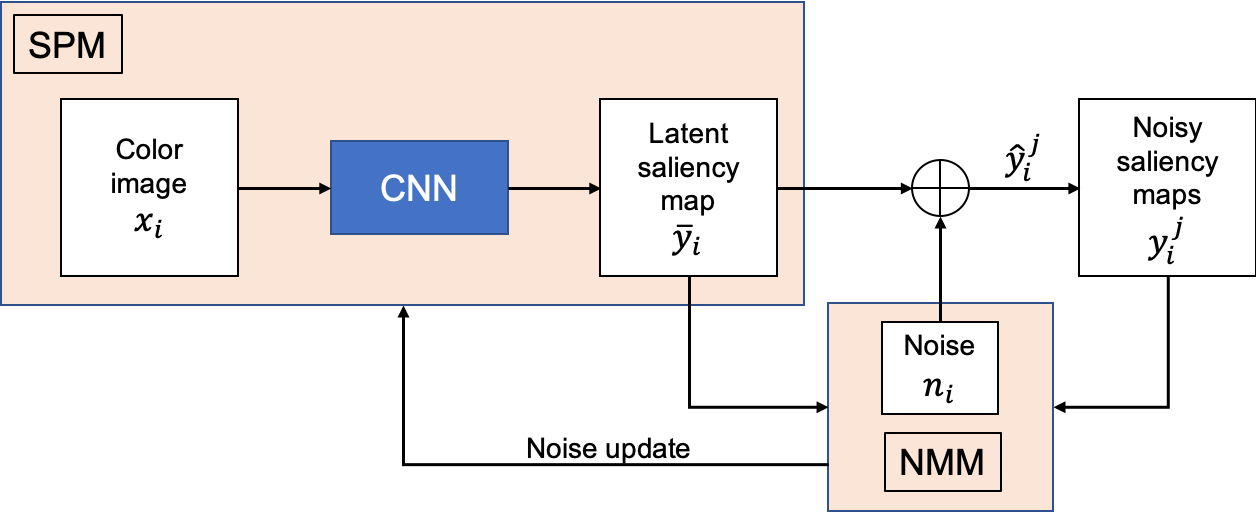
\includegraphics[width=0.8\linewidth]{fig1.png}
  \caption{Schematic representation of our deep unsupervised saliency detection framework, which consists of a latent saliency prediction module and a noise modeling module.}
  \label{fig:scheme}
\end{figure}

\subsection{Loss Function}
As we mentioned before, one of the central aspects of the work proposed in \cite{zhang2018} is the loss function of their framework, which is one of the main contributions of the work and essential to the end-to-end training feature. Given the variance $\Sigma$ of the zero-mean Gaussian distribution, where the noise $\boldsymbol{n}^{j}_i \sim\boldsymbol{q}_i(\Sigma)$ is sampled from, and the parameter $\Theta$ of the CNN, that predicts the saliency map, $\bar{\boldsymbol{y}_i} = f(\boldsymbol{x}_i, \Theta)$, the loss function for our framework is:

\begin{equation}
  \mathcal{L}(\Theta, \Sigma) = \mathcal{L}_{\textnormal{pred}}(\Theta, \Sigma) + \lambda \cdot \mathcal{L}_{\textnormal{noise}}(\Theta, \Sigma),
  \label{eq:loss_fn}
\end{equation}

where $\lambda$ is the regularization term, which balances both losses terms. With an increase in the noise, modeling variance makes prediction loss large and decrease noise loss. Meanwhile, keeping the variance lower will decrease the prediction loss but increase the noise loss \cite{zhang2018}. Therefore, optimizing the loss function is to achieve a balance between the NMM, which increases generalization, and the SPM with good accuracy. We define in detail the losses for both SPM and NMM below. 

\subsubsection{Saliency Prediction}

The main component of the SPM is a CNN, that applies a traditional cross-entropy loss, which is computed element-wisely at a pixel level across the images. Given an $m \times n$ image $\boldsymbol{x}_i$, its predicted label $\hat{y}$, and its ground truth label $y$, the cross-entropy loss, $L_{CE}$, is: 

\begin{equation}
  L_{CE} = - \left( y \cdot \log{(\hat{y})} + (1 - y) \cdot \log{(1 - \hat{y})} \right)
  \label{eq:cross-entropy}
\end{equation}

Further, the SPM loss, $\mathcal{L}_{pred}(\Theta,\Sigma)$, is: 

\begin{equation}
  \mathcal{L}_{\textnormal{pred}}(\Theta,\Sigma) = \sum_{i=1}^{N}\sum_{j=1}^{M}\sum_{m,n} L_{CE} \left(\textbf{y}_{i,mn}^{i}, \hat{\textbf{y}}_{i,mn}^{j} \right),
  \label{eq:pred_loss}
\end{equation}
where $\textbf{y}_{i,mn}^{i}$ and $\hat{\textbf{y}}_{i,mn}^{i}$ is our predicted noisy saliency map and pseudo ground truth saliency maps (\ie unsupervised methods), respectively. The first is computed by $\boldsymbol{\hat{y}}_i^{j} = \bar{\boldsymbol{y}_i} + \boldsymbol{n}^{j}_i$ and truncated to the interval $[0,1]$.

\subsubsection{Noise Modeling}
\label{section:NMM}

For each image $\boldsymbol{x}_i$, an empirical noise can be computed from the saliency map outputed from the SPM, $\hat{\boldsymbol{n}}^j_i = \boldsymbol{y}_i^{j} - \bar{\boldsymbol{y}_i}$. Assuming the empirical noise follows a zero-mean Gaussian probability distribution, $p(\hat{\Sigma}_i)$, which the complete set of parameters being $\hat{\Sigma} = \{\hat{\sigma_{i, mn}}\}$, with the variance of each pixel denoted by $\sigma_{i, mn}$.

Since it is intractable to estimate the true posterior distribution $q(\Sigma)$, the original work proposed to approximate it by sequentially optimizing the parameters of the zero-mean Gaussian prior distribution \cite{zhang2018}. In addition, the noise is randomly produced based on an parameters set $\Sigma$. Since given an image $\boldsymbol{x}_i$ and the SPM parameters $\Theta$, the NMM works as a probabilistic encoder that generates a distribution over possible values of noise $n$. The procedure has two stages: (1) a noise map $n_i$ is produced from some prior $q(\Sigma^*)$, and (2) a noise map $\hat{n}_i^j$ is generated and the corresponding pixel variances $\hat{\sigma}_i$ are estimated.

Hence, we want to maximize the agreement between the true distribution $q(\Sigma_i)$ of the NMM and the approximated empirical distribution of noise $p(\hat{\Sigma}_i)$ by minimizing the forward Kullback-Leibler (KL) divergence. Thus, our NMM loss, $\mathcal{L}_{\textnormal{noise}}$, is: 

\begin{equation}
  \mathcal{L}_{\textnormal{noise}}(\Theta,\Sigma) = \sum_{i=1}^N \mathrm{KL} \left(q(\Sigma_i) || p(\hat{\Sigma}_i) \right)
  \label{eq:noise_loss}
\end{equation}

Since a zero-mean Gaussin distribution is our noise model prior, the KL divergence has a closed-form as follows:

\begin{equation}
  \mathrm{KL} \left(q(\sigma) || p(\hat{\sigma}) \right) = \log \left( \dfrac{\hat{\sigma}}{\sigma} \right) + \dfrac{\sigma^2 + (\mu - \hat{\mu})^2}{2 \cdot \hat{\sigma}^2} - \dfrac{1}{2}
  \label{eq:kl_closed}
\end{equation}

Based on the previous equation, we derive an update rule for the variances of the noise at pixel level of each $m \times n$ image, as described in \cite{zhang2018}, as follows: 

\begin{equation}
  (\sigma^{t+1}_i)^2 = (\sigma^{t}_i)^2 + \alpha \left( (\hat{\sigma}^t_i)^2 - (\sigma^{t}_i)^2 \right),
  \label{eq:update}
\end{equation}
where $\alpha$ is the step size and was set to $0.01$ as in \cite{zhang2018}.

Since each image has a corresponding noise map, it is difficult to converge simultaneously the parameters of SPM ($\Theta$) and NMM ($\Sigma$). As a solution, we update them in rounds. At the first round, noise variance is initialized to be zero, we train the CNN for one epoch, using Eqs. \eqref{eq:cross-entropy} and \eqref{eq:pred_loss}, and we update the NMM using Eq. \eqref{eq:update}. Based on the variance of the saliency prediction and noisy labels, then the noise variance is updated for each image and retrain the network. Using the updated noise variance sampled from NMM as initialization, the next round can proceed. The next $i$ rounds, we train SPM on unsupervised labels for 20 epochs, using Eq. \eqref{eq:loss_fn}, and we update the NMM using Eq. \eqref{eq:update}.

\subsection{Architecture and Implementation}

We build our SPM upon the DeepLab network \cite{Deeplab}, where a pre-trained ResNet-101 \cite{ResNet101} for image classification is re-purposed with modifications in its last classifier layer to convolutional layers. 

The input of our model are rescaled images ($x_i$) and transformations ($y_i^j$) of $256 \times 256$. For training, the noise model is used to update the predicted saliency map $\hat{y}_i^j$, and it is not considered in the validation and testing stages, where our SPM outputs the latent salient map ($\bar{y_i}$).

\section{Experiments}

We try to minimize the loss function of the framework in the training process using different types of optimizers (\ie Adam and SGD) and learning rate schedulers (\ie StepLR and ReduceLROnPlateau) with the MSRA-B dataset and the four image transformations. The dataset, unsupervised image transformation, the evaluation metrics, and the baseline experiments are described below.

\subsection{Dataset}

In our project, we propose to reproduce the work of \cite{zhang2018} with MSRA-B dataset \cite{wang2017}, 5000 images with pixel-accurate object labeling, which most images only have one salient object. One example of the dataset with its label and unsupervised transformations are shown in Figure \ref{fig:samples}. Further, we split the MSRA-B dataset in 2500, 500, and 2000 images as training, validation, and test sets respectively.

\begin{figure}[h]
  \begin{subfigure}{.33\textwidth}
    \centering
    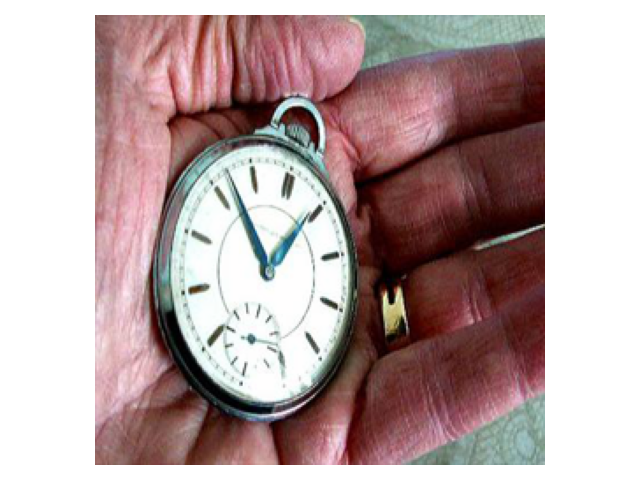
\includegraphics[width=\linewidth]{./samples/dataset.png}
    \caption{Original}
    \label{fig:sample}
  \end{subfigure}
  % \hfill
  \begin{subfigure}{.33\textwidth}
    \centering
    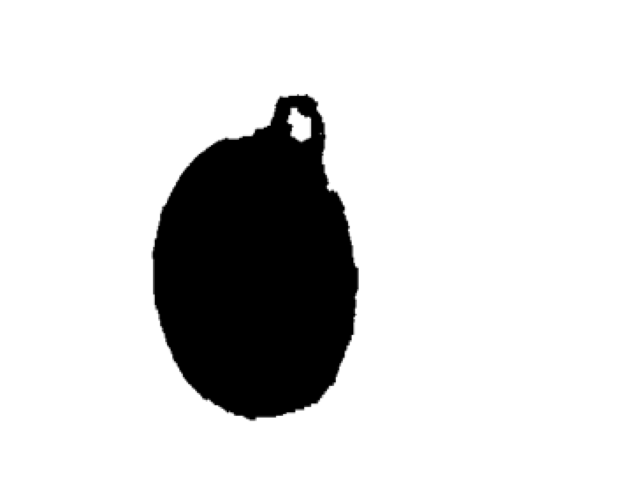
\includegraphics[width=\linewidth]{./samples/label.png}
    \caption{Ground truth label}
    \label{fig:label}
  \end{subfigure}
  % \hfill
  \begin{subfigure}{.33\textwidth}
    \centering
    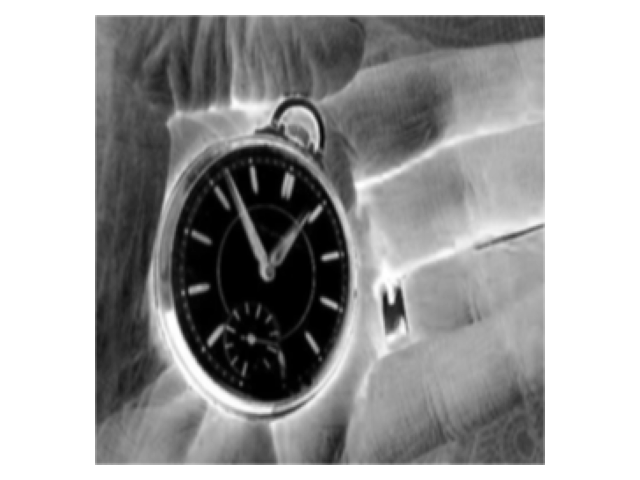
\includegraphics[width=\linewidth]{./samples/ft.png}
    \caption{FT transformation}
    \label{fig:ft}
  \end{subfigure}
  % \hfill
  \begin{subfigure}{.33\textwidth}
    \centering
    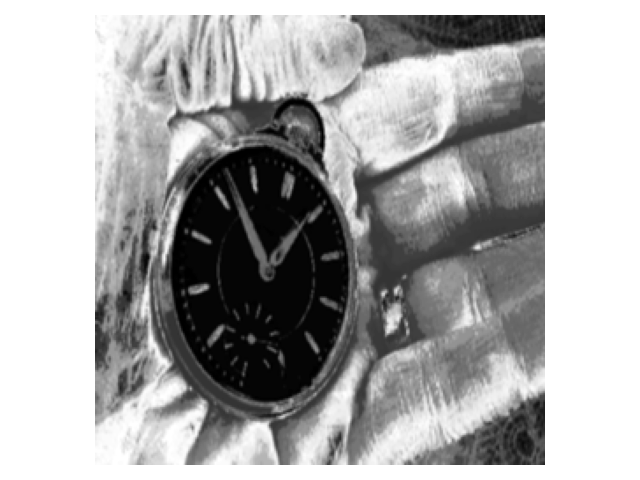
\includegraphics[width=\linewidth]{./samples/hc.png}
    \caption{HC transformation}
    \label{fig:hc}
  \end{subfigure}
  % \hfill
  \begin{subfigure}{.33\textwidth}
    \centering
    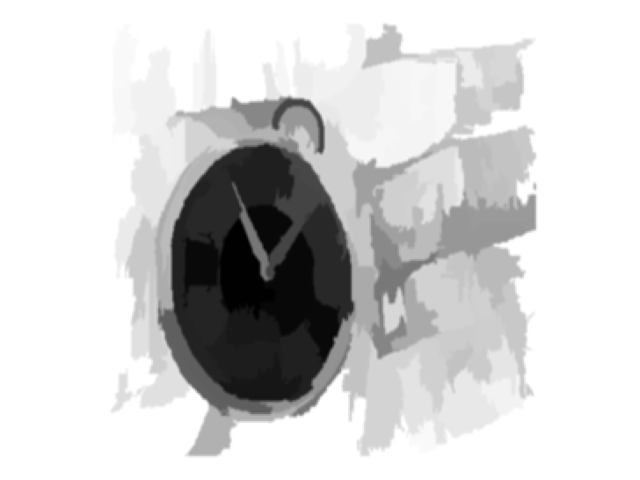
\includegraphics[width=\linewidth]{./samples/rc.png}
    \caption{RC transformation}
    \label{fig:rc}
  \end{subfigure}
  % \hfill
  \begin{subfigure}{.33\textwidth}
    \centering
    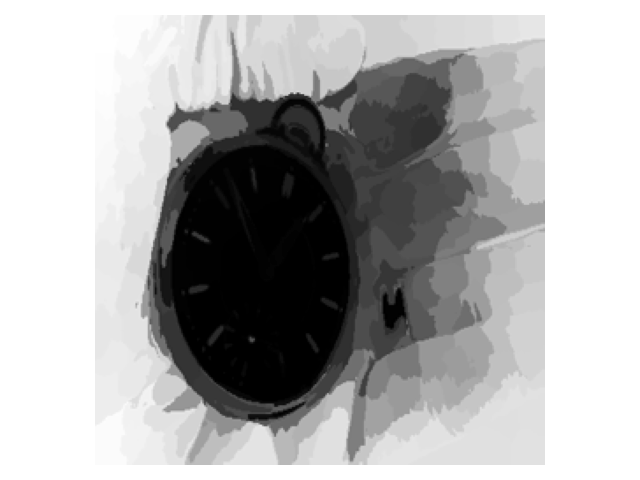
\includegraphics[width=\linewidth]{./samples/rdb.png}
    \caption{RBD transformation}
    \label{fig:rbd}
  \end{subfigure}
  % \hfill
  \caption{An example from the dataset and its ground truth saliency map and unsupervised transformations.}
  \label{fig:samples}
\end{figure}

\subsection{Images Transformations}

In this project, we applied four unsupervised transformations in our images from dataset MSRA-B (Figures \ref{fig:ft}, \ref{fig:hc}, \ref{fig:rc} and \ref{fig:rbd}). % just for training set (2500 images)
The first one is the Frequency-Tuned (FT), described by \cite{FT}, which exploits features of color and luminance, is simple to implement, computationally efficient, and in the paper is used to output full resolution saliency maps with well-defined boundaries of salient objects. 
The second and third one is Histogram Based Contrast (HC) and Region-Based Contrast (RC), both described in \cite{HCRC}, which simultaneously evaluates global contrast differences and spatially weighted coherence scores, being simple, efficient, naturally multi-scalable, and produces full-resolution, high-quality saliency maps. 
The last one is Robust Background Detection (RBD), which characterizes the spatial layout of image regions with respect to image boundaries and has an intuitive geometrical interpretation, as is described in \cite{RBD}.

\subsection{Evaluation Metrics}

We evaluate our model with a set of evaluation metrics, including mean absolute error (MAE; Eq. \eqref{eq:mae}), Precision (P; Eq. \eqref{eq:precision}), Recall (R; Eq. \eqref{eq:recall}) and F-measure (F$_\beta$; Eq. \eqref{eq:fmeasure}). The MAE represents the dissimilarity between the estimated binary and the ground truth saliency map.

\begin{equation}
  MAE = \dfrac{1}{N} \sum_{j=1}^{N} |y_j - \hat{y}_j|,
  \label{eq:mae}
\end{equation}
where $N$ is the number of images in the set, $y_j$ is the ground truth saliency maps and $\hat{y}_j$ is the predicted binary saliency map.

\begin{equation}
 P = \dfrac{TP}{TP + FP}
 \label{eq:precision}
\end{equation}

\begin{equation}
  R = \dfrac{TP}{TP + FN},
  \label{eq:recall}
\end{equation}
where $TP$ is the number of true positives, $FP$ is the number of false positives and $FN$ is the number of false negatives.

\begin{equation}
  F_\beta = (1 + \beta^2) \dfrac{P \cdot R}{\beta^2 \cdot P + R},
  \label{eq:fmeasure}
\end{equation}
where $P$ is the precision that corresponds to the correctly detected salient pixels, $R$ is the recall that corresponds to the fraction of detected salient pixels \wrt the ground truth salient pixels and $\beta = 0.3$.

\subsection{Baseline Experiments}

We explored three different baseline experiments based on the utilization of the multiple saliency maps of our model. The description of each baseline experiment is provided below.

\begin{itemize}
  \item \textbf{Baseline Experiment 1 (Real):} The SPM is trained directly with the clean ground truth labels provided by the MSRA-B dataset;
  \item \textbf{Baseline Experiment 2 (Noise):} The SPM is trained on our four noisy unsupervised labels (FT, HC, RC, and RBD);
  \item \textbf{Baseline Experiment 3 (Average):} Instead of training the SPM with our noisy unsupervised labels, we train the average saliency map of those unsupervised labels as pseudo ground truth.
\end{itemize}

In the complete model (denoted by \textbf{Complete}), the SPM and NMM are trained together with the procedure previously described in Section \ref{section:NMM}. However, we just trained their experiments with one round.

Finally, our baseline experiments and complete model are trained for 20 epochs. As mentioned above, we explored different optimizers and learning rate schedulers and their parameters are as follows. The Adam optimizer with betas of $0.9$ and $0.99$ and base learning rate of $1e-3$ and the SGD optimizer with momentum $0.9$ and base learning rate of $1e-3$. The StepLR decays the learning rate of each parameter group by 0.9 every 10 epochs and the ReduceLROnPlateau decays the learning rate by 0.9 when the validation loss has stopped improved for 10 epochs and waits for one epoch before resuming normal operation after the learning rate has been reduced.

\section{Results}

\subsection{Loss function}

The loss functions, Eq.~\eqref{eq:loss_fn}, per epoch at the training stage, for our baseline experiments and complete model, are shown in Figure \ref{fig:loss}. We noticed that the loss function decreases and smoothly stabilizes in all scenarios, which is the expected behavior. This minimization of the loss function indicates that the baseline experiments and our framework are learning better saliency detection maps. In addition, our framework is also learning better parameters for the NMM, from which the noise is sampled.

\begin{figure}[h]
  \centering
  %
  % Real
  \begin{subfigure}[c]{0.245\textwidth}
    \centering
      \subcaption*{Adam}
      \myrowlabel{Real}
      \raisebox{-.5\height}{\includegraphics[width=0.85\textwidth]
      {Real/Adam/StepLR/images/train/Loss.png}}\\
      \myrowlabel{Noise}
      \raisebox{-.5\height}{\includegraphics[width=0.85\textwidth]
      {Noise/Adam/StepLR/images/train/Loss.png}}\\
      \myrowlabel{Average}
      \raisebox{-.5\height}{\includegraphics[width=0.85\textwidth]
      {Average/Adam/StepLR/images/train/Loss.png}}
      \myrowlabel{Complete}
      \raisebox{-.5\height}{\includegraphics[width=0.85\textwidth]
      {Complete/Adam/StepLR/images/train/Loss.png}}
    \subcaption*{StepLR}
  \end{subfigure}
  %
  % Noise
  \begin{subfigure}[c]{0.245\textwidth}
    \centering
      \subcaption*{Adam}
      \includegraphics[width=0.85\textwidth]  
      {Real/Adam/ReduceLROnPlateau/images/train/Loss.png}
      \includegraphics[width=0.85\textwidth]
      {Noise/Adam/ReduceLROnPlateau/images/train/Loss.png}
      \includegraphics[width=0.85\textwidth]
      {Average/Adam/ReduceLROnPlateau/images/train/Loss.png}
      \includegraphics[width=0.85\textwidth]
      {Complete/Adam/ReduceLROnPlateau/images/train/Loss.png}
      \subcaption*{ReduceLROnPlateau}
  \end{subfigure}
  %
  % Average
  \begin{subfigure}[c]{0.245\textwidth}
    \centering
      \subcaption*{SGD}
      \includegraphics[width=0.85\textwidth]  
      {Real/SGD/StepLR/images/train/Loss.png}
      \includegraphics[width=0.85\textwidth]
      {Noise/SGD/StepLR/images/train/Loss.png}
      \includegraphics[width=0.85\textwidth]
      {Average/SGD/StepLR/images/train/Loss.png}
      \includegraphics[width=0.85\textwidth]
      {Complete/SGD/StepLR/images/train/Loss.png}
      \subcaption*{StepLR}
  \end{subfigure}
  %
  % Complete
  \begin{subfigure}[c]{0.245\textwidth}
    \centering
      \subcaption*{SGD}
      \includegraphics[width=0.85\textwidth]  
      {Real/SGD/ReduceLROnPlateau/images/train/Loss.png}
      \includegraphics[width=0.85\textwidth]
      {Noise/SGD/ReduceLROnPlateau/images/train/Loss.png}
      \includegraphics[width=0.85\textwidth]
      {Average/SGD/ReduceLROnPlateau/images/train/Loss.png}
      \includegraphics[width=0.85\textwidth]
      {Complete/SGD/ReduceLROnPlateau/images/train/Loss.png}
      \subcaption*{ReduceLROnPlateau}
  \end{subfigure}
  %
  \caption{Training loss function for each baseline experiment and our framework with different optimizers and learning rate schedulers on MSRA-B dataset. The experiment, the optimizer and the learning rate scheduler are shown in the right, top and bottom of the figure, respectively.}
  \label{fig:loss}
\end{figure}

\subsection{Evaluation Metrics}
\label{section:evaluation_metrics}

Here, we compare the evaluation metrics (MAE and F-measure) between our baseline experiments and complete models, which are shown in Table \ref{tab:comp}. The combination of SGD optimizer and ReduceLROnPlateau scheduler showed the best evaluation metrics for all baseline experiments and our framework except for Average that Adam optimizer had slightly better metrics, agreeing with the implementation in \cite{zhang2018}. Our framework outperforms both Noise and Average experiments, showing that our framework works better with unsupervised labels as pseudo ground truth. Further, the Average also outperforms the Noise experiment, because the first has 3000 averaged training unsupervised label, which probably better identifies the salient object than 12000 training unsupervised labels; and we suggest that the chosen unsupervised saliency methods are complementary to some extent, since averaging than yield better supervision than each one of them individually. Unexpectedly, our framework presented a worse performance than the Real experiment, which is trained with a ground truth saliency map. This indicates that our selection of unsupervised saliency methods could not have been the best option, which leads to a worse performance when compared to \cite{zhang2018}.

\begin{table}[h]
  \centering
  \begin{tabular}{|l|c|c|c|c|c|c|c|c|}
  \hline
  \multicolumn{1}{|c|}{\textbf{Optimizer}} & \multicolumn{4}{c|}{\textbf{Adam}} & \multicolumn{4}{c|}{\textbf{SGD}} \\ \hline
  \multicolumn{1}{|c|}{\textbf{Scheduler}} & \multicolumn{2}{c|}{\textbf{StepLR}} & \multicolumn{2}{c|}{\textbf{ReduceLROnPlateau}} & \multicolumn{2}{c|}{\textbf{StepLR}} & \multicolumn{2}{c|}{\textbf{ReduceLROnPlateau}} \\ \hline
  \textbf{Experiment} & \textit{\textbf{$F_\beta$}} & \textit{\textbf{MAE}} & \textit{\textbf{$F_\beta$}} & \textit{\textbf{MAE}} & \textit{\textbf{$F_\beta$}} & \textit{\textbf{MAE}} & \textit{\textbf{$F_\beta$}} & \textit{\textbf{MAE}} \\ \hline
  \textit{\textbf{Real}} & 0.8934 & 0.0518 & 0.8925 & 0.0520 & 0.9248 & 0.037 & 0.9256 & 0.036 \\ \hline
  \textit{\textbf{Noise}} & 0.6514 & 0.1400 & 0.5937 & 0.1567 & 0.6640 & 0.1389 & 0.6682 & 0.1376 \\ \hline
  \textit{\textbf{Average}} & 0.6897 & 0.1359 & 0.7316 & 0.1227 & 0.7061 & 0.1317 & 0.7287 & 0.1267 \\ \hline
  \textit{\textbf{Complete}} & 0.6904 & 0.1432 & 0.7013 & 0.1384 & 0.7810 & 0.1043 & 0.7888 & 0.1033 \\ \hline
  \end{tabular}
  \caption{Perfomance of each baseline experiment and our framework with different optimizers and learning rate schedulers on MSRA-B dataset.}
  \label{tab:comp}
\end{table}

\subsection{Saliency Maps}

A predicted saliency map for the baseline experiments and our framework with the SGD optimizer and the ReduceLROnPlateau scheduler (best combination), which achieved the best evaluation metrics (MAE and F-measure), are shown in Figure \ref{fig:comp_images} with their original image and their ground truth saliency map.

\begin{figure}[h]
  \centering
  % Images
  \begin{subfigure}[c]{0.16\textwidth}
    \centering
      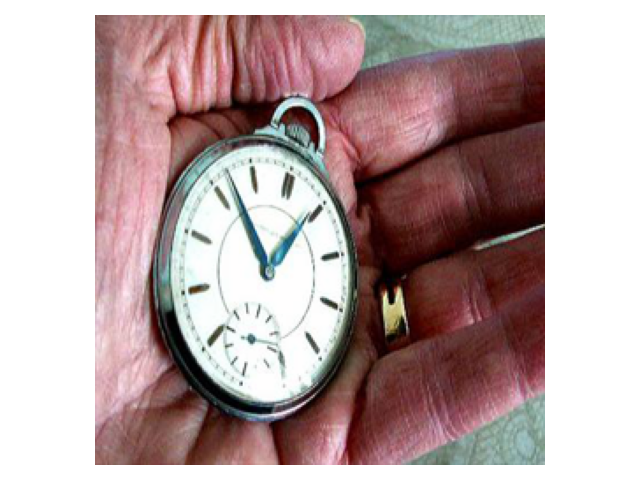
\includegraphics[width=\textwidth]
      {Real/SGD/ReduceLROnPlateau/images/0_real.png}
    \subcaption*{Images}
  \end{subfigure}
  %
  % Ground truth
  \begin{subfigure}[c]{0.16\textwidth}
    \centering
      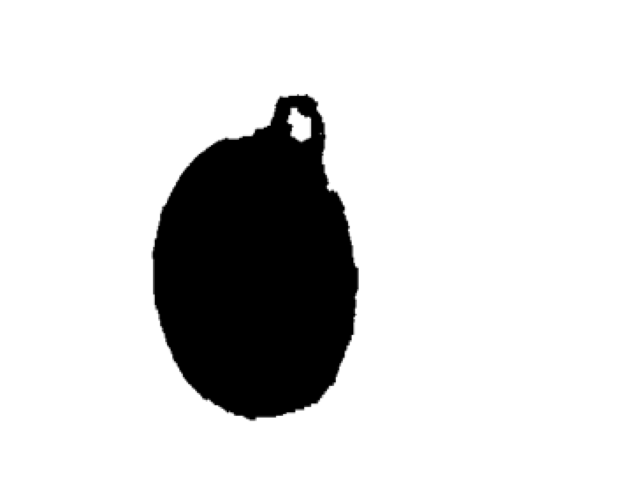
\includegraphics[width=\textwidth]  
      {Real/SGD/ReduceLROnPlateau/images/0_gt.png}
      \subcaption*{Ground truth}
  \end{subfigure}
  %
  % Real
  \begin{subfigure}[c]{0.16\textwidth}
    \centering
      \includegraphics[width=\textwidth]  
      {Real/SGD/ReduceLROnPlateau/images/0_pred_binary_20.png}
      \subcaption*{Real}
  \end{subfigure}
  %
  % Noise
  \begin{subfigure}[c]{0.16\textwidth}
    \centering
    \includegraphics[width=\textwidth]  
    {Noise/SGD/ReduceLROnPlateau/images/0_pred_binary_20.png}
    \subcaption*{Noise}
  \end{subfigure}
  %
  % Average
  \begin{subfigure}[c]{0.16\textwidth}
    \centering
    \includegraphics[width=\textwidth]  
    {Average/SGD/ReduceLROnPlateau/images/0_pred_binary_20.png}
    \subcaption*{Average}
  \end{subfigure}
  %
  % Complete
  \begin{subfigure}[c]{0.16\textwidth}
    \centering
    \includegraphics[width=\textwidth]  
    {Complete/SGD/ReduceLROnPlateau/images/0_pred_binary_20.png}
    \subcaption*{Complete}
  \end{subfigure}
  %
  \caption{Comparison of a predicted saliency between the baseline experiments and our framework.}
  \label{fig:comp_images}
\end{figure}

Additionally, some examples from the validation set are shown for each baseline experiment and our framework, with the SGD optimizer and the ReduceLROnPlateau scheduler, below.

\subsubsection{Real}

The saliency maps with the SPM trained directly with the clean ground truth labels are shown in Figure \ref{fig:real_sm}.

\begin{figure}[p]
  \centering
  % Images
  \begin{subfigure}[c]{0.19\textwidth}
    \centering
      \includegraphics[width=\textwidth]{Real/SGD/ReduceLROnPlateau/images/1_real.png}
      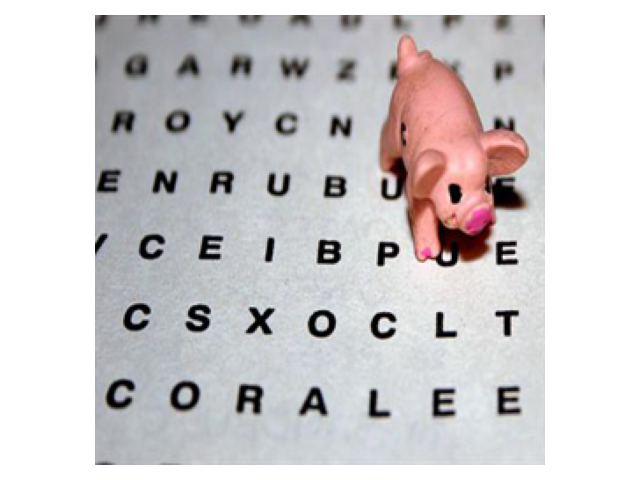
\includegraphics[width=\textwidth]{Real/SGD/ReduceLROnPlateau/images/2_real.png}
      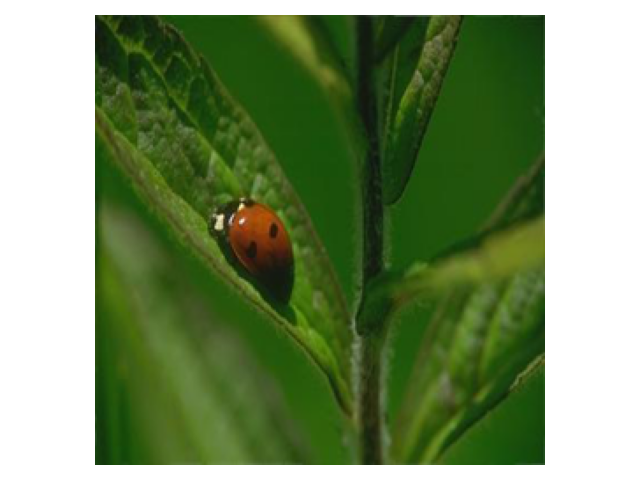
\includegraphics[width=\textwidth]{Real/SGD/ReduceLROnPlateau/images/3_real.png}
      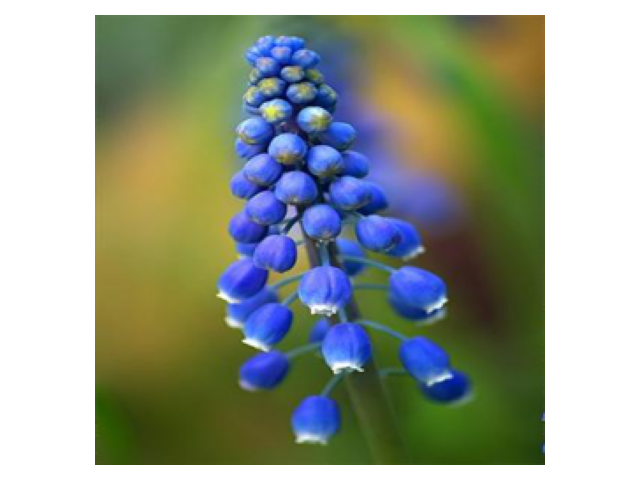
\includegraphics[width=\textwidth]{Real/SGD/ReduceLROnPlateau/images/4_real.png}
    \subcaption*{Images}
  \end{subfigure}
  %
  % Ground truth
  \begin{subfigure}[c]{0.19\textwidth}
    \centering
      
\includegraphics[width=\textwidth]{Real/SGD/ReduceLROnPlateau/images/1_gt.png}
      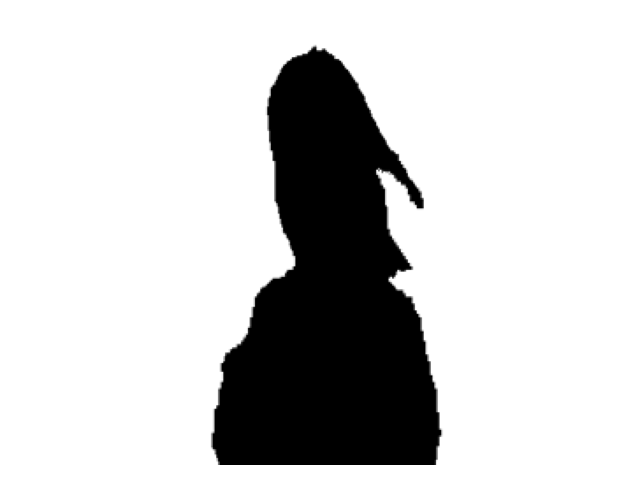
\includegraphics[width=\textwidth]{Real/SGD/ReduceLROnPlateau/images/2_gt.png}
      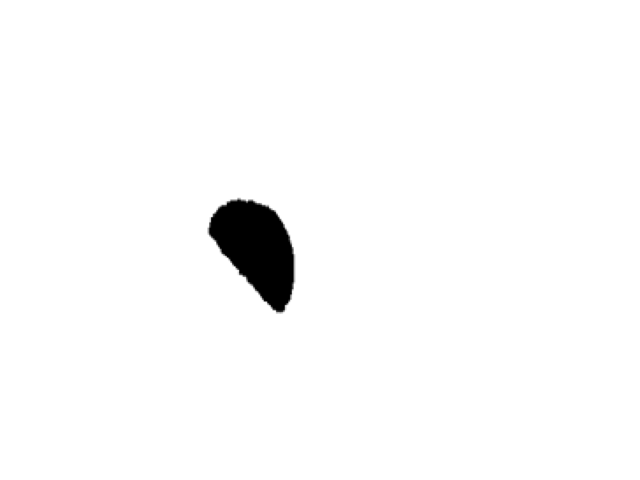
\includegraphics[width=\textwidth]{Real/SGD/ReduceLROnPlateau/images/3_gt.png}
      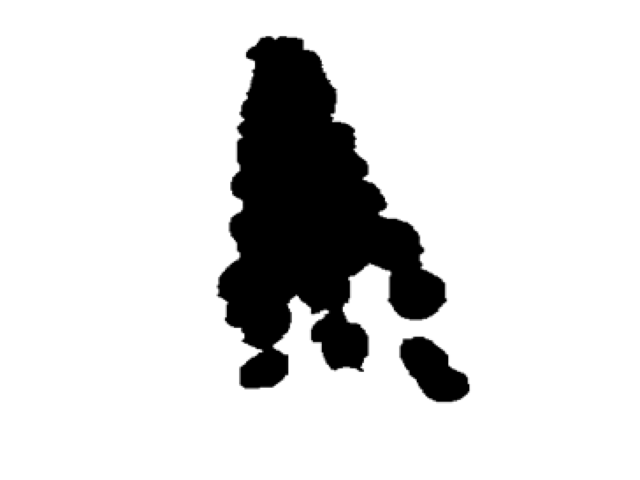
\includegraphics[width=\textwidth]{Real/SGD/ReduceLROnPlateau/images/4_gt.png}
      \subcaption*{Ground truth}
  \end{subfigure}
  %
  % 1st epoch
  \begin{subfigure}[c]{0.19\textwidth}
    \centering
    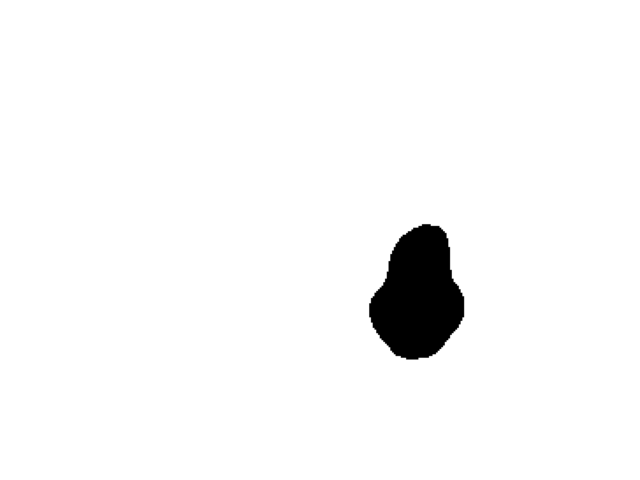
\includegraphics[width=\textwidth]{Real/SGD/ReduceLROnPlateau/images/1_pred_binary_1.png}
    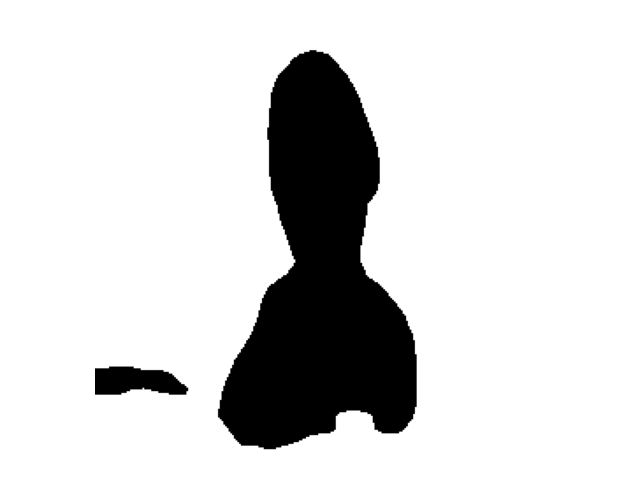
\includegraphics[width=\textwidth]{Real/SGD/ReduceLROnPlateau/images/2_pred_binary_1.png}
    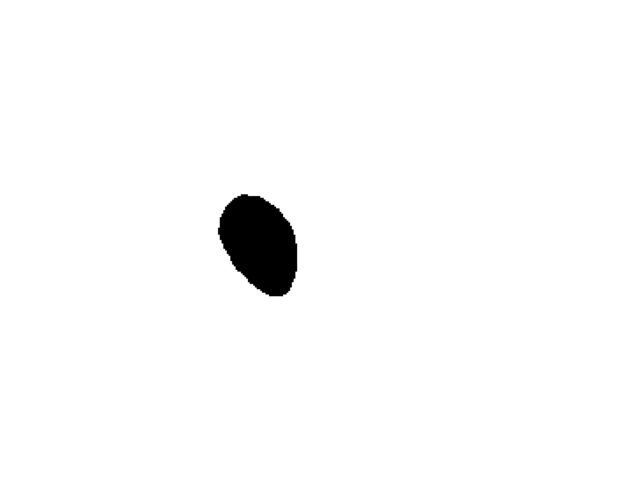
\includegraphics[width=\textwidth]{Real/SGD/ReduceLROnPlateau/images/3_pred_binary_1.png}
    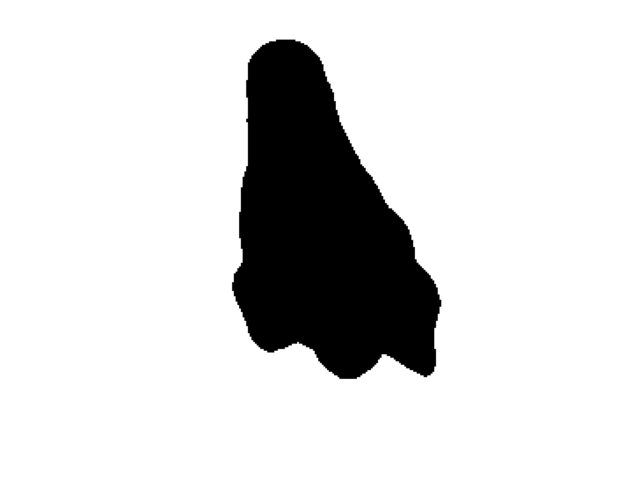
\includegraphics[width=\textwidth]{Real/SGD/ReduceLROnPlateau/images/4_pred_binary_1.png}
      \subcaption*{Epoch 1}
  \end{subfigure}
  %
  % 10th epoch
  \begin{subfigure}[c]{0.19\textwidth}
    \centering
    \includegraphics[width=\textwidth]{Real/SGD/ReduceLROnPlateau/images/1_pred_binary_10.png}
    \includegraphics[width=\textwidth]{Real/SGD/ReduceLROnPlateau/images/2_pred_binary_10.png}
    \includegraphics[width=\textwidth]{Real/SGD/ReduceLROnPlateau/images/3_pred_binary_10.png}
    \includegraphics[width=\textwidth]{Real/SGD/ReduceLROnPlateau/images/4_pred_binary_10.png}
    \subcaption*{Epoch 10}
  \end{subfigure}
  %
  % 20th epoch
  \begin{subfigure}[c]{0.19\textwidth}
    \centering
    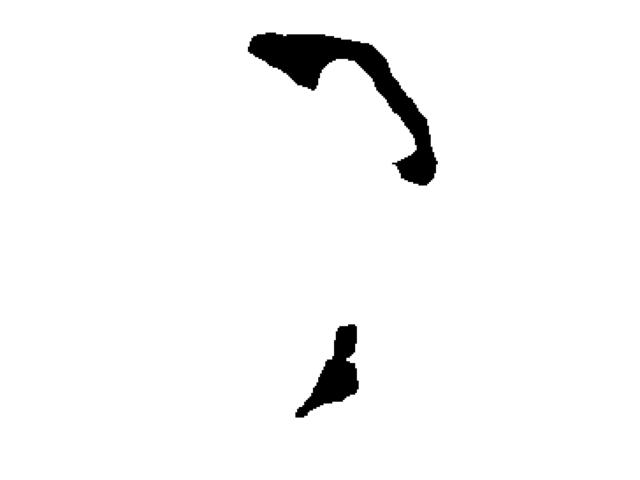
\includegraphics[width=\textwidth]{Real/SGD/ReduceLROnPlateau/images/1_pred_binary_20.png}
    
\includegraphics[width=\textwidth]{Real/SGD/ReduceLROnPlateau/images/2_pred_binary_20.png}
    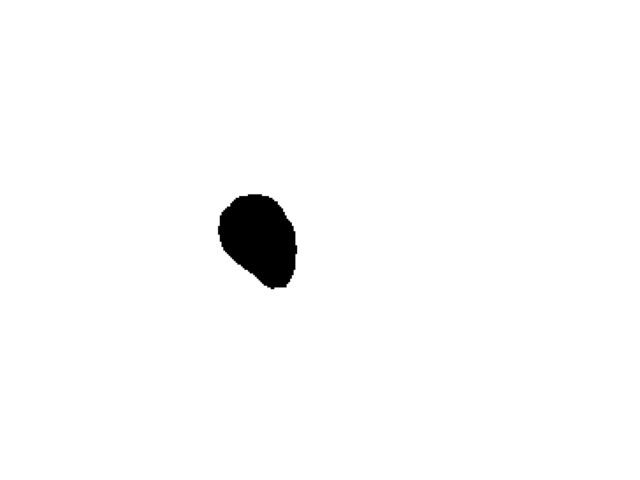
\includegraphics[width=\textwidth]{Real/SGD/ReduceLROnPlateau/images/3_pred_binary_20.png}
    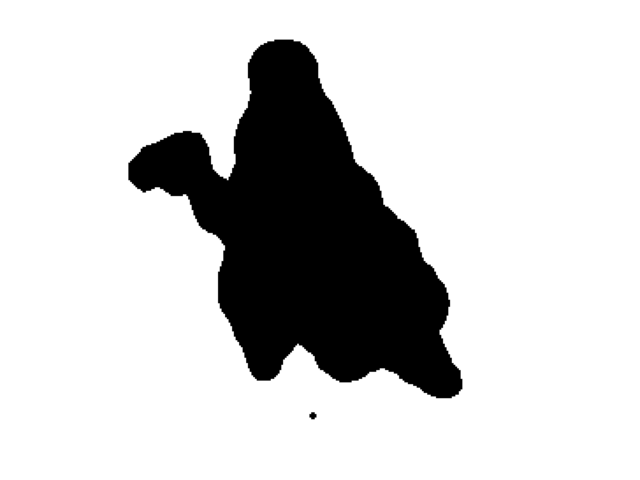
\includegraphics[width=\textwidth]{Real/SGD/ReduceLROnPlateau/images/4_pred_binary_20.png}
    \subcaption*{Epoch 20}
  \end{subfigure}
  %
  \caption{Comparison between the predicted saliency maps of the Real baseline experiment.}
  \label{fig:real_sm}
\end{figure}

\subsubsection{Noise}

The saliency maps of the SPM, trained with our four unsupervised saliency methods (FT, HC, RC and RBD) as ground truth labels, are shown in Figure \ref{fig:noise_sm}. 


\begin{figure}[p]
  \centering
  % Images
  \begin{subfigure}[c]{0.19\textwidth}
    \centering
      \includegraphics[width=\textwidth]{Noise/SGD/ReduceLROnPlateau/images/1_real.png}
      \includegraphics[width=\textwidth]{Noise/SGD/ReduceLROnPlateau/images/2_real.png}
      \includegraphics[width=\textwidth]{Noise/SGD/ReduceLROnPlateau/images/3_real.png}
      \includegraphics[width=\textwidth]{Noise/SGD/ReduceLROnPlateau/images/4_real.png}
    \subcaption*{Images}
  \end{subfigure}
  %
  % Ground truth
  \begin{subfigure}[c]{0.19\textwidth}
    \centering
      \includegraphics[width=\textwidth]{Noise/SGD/ReduceLROnPlateau/images/1_gt.png}
      \includegraphics[width=\textwidth]{Noise/SGD/ReduceLROnPlateau/images/2_gt.png}
      \includegraphics[width=\textwidth]{Noise/SGD/ReduceLROnPlateau/images/3_gt.png}
      \includegraphics[width=\textwidth]{Noise/SGD/ReduceLROnPlateau/images/4_gt.png}
      \subcaption*{Ground truth}
  \end{subfigure}
  %
  % 1st epoch
  \begin{subfigure}[c]{0.19\textwidth}
    \centering
    \includegraphics[width=\textwidth]{Noise/SGD/ReduceLROnPlateau/images/1_pred_binary_1.png}
    \includegraphics[width=\textwidth]{Noise/SGD/ReduceLROnPlateau/images/2_pred_binary_1.png}
    \includegraphics[width=\textwidth]{Noise/SGD/ReduceLROnPlateau/images/3_pred_binary_1.png}
    \includegraphics[width=\textwidth]{Noise/SGD/ReduceLROnPlateau/images/4_pred_binary_1.png}
      \subcaption*{Epoch 1}
  \end{subfigure}
  %
  % 10th epoch
  \begin{subfigure}[c]{0.19\textwidth}
    \centering
    \includegraphics[width=\textwidth]{Noise/SGD/ReduceLROnPlateau/images/1_pred_binary_10.png}
    \includegraphics[width=\textwidth]{Noise/SGD/ReduceLROnPlateau/images/2_pred_binary_10.png}
    \includegraphics[width=\textwidth]{Noise/SGD/ReduceLROnPlateau/images/3_pred_binary_10.png}
    \includegraphics[width=\textwidth]{Noise/SGD/ReduceLROnPlateau/images/4_pred_binary_10.png}
    \subcaption*{Epoch 10}
  \end{subfigure}
  %
  % 20th epoch
  \begin{subfigure}[c]{0.19\textwidth}
    \centering
    \includegraphics[width=\textwidth]{Noise/SGD/ReduceLROnPlateau/images/1_pred_binary_20.png}
    \includegraphics[width=\textwidth]{Noise/SGD/ReduceLROnPlateau/images/2_pred_binary_20.png}
    \includegraphics[width=\textwidth]{Noise/SGD/ReduceLROnPlateau/images/3_pred_binary_20.png}
    \includegraphics[width=\textwidth]{Noise/SGD/ReduceLROnPlateau/images/4_pred_binary_20.png}
    \subcaption*{Epoch 20}
  \end{subfigure}
  %
  \caption{Comparison between the predicted saliency maps of the Noise baseline experiment.}
  \label{fig:noise_sm}
\end{figure}

\subsubsection{Average}

The saliency maps of the SPM, trained with the average saliency map of our four unsupervised saliency methods (FT, HC, RC and RBD) as ground truth labels, are illustrated in Figure \ref{fig:average_sm}.

\begin{figure}[p]
  \centering
  % Images
  \begin{subfigure}[c]{0.19\textwidth}
    \centering
      \includegraphics[width=\textwidth]{Average/SGD/ReduceLROnPlateau/images/1_real.png}
      \includegraphics[width=\textwidth]{Average/SGD/ReduceLROnPlateau/images/2_real.png}
      \includegraphics[width=\textwidth]{Average/SGD/ReduceLROnPlateau/images/3_real.png}
      \includegraphics[width=\textwidth]{Average/SGD/ReduceLROnPlateau/images/4_real.png}
    \subcaption*{Images}
  \end{subfigure}
  %
  % Ground truth
  \begin{subfigure}[c]{0.19\textwidth}
    \centering
      \includegraphics[width=\textwidth]{Average/SGD/ReduceLROnPlateau/images/1_gt.png}
      \includegraphics[width=\textwidth]{Average/SGD/ReduceLROnPlateau/images/2_gt.png}
      \includegraphics[width=\textwidth]{Average/SGD/ReduceLROnPlateau/images/3_gt.png}
      \includegraphics[width=\textwidth]{Average/SGD/ReduceLROnPlateau/images/4_gt.png}
      \subcaption*{Ground truth}
  \end{subfigure}
  %
  % 1st epoch
  \begin{subfigure}[c]{0.19\textwidth}
    \centering
    \includegraphics[width=\textwidth]{Average/SGD/ReduceLROnPlateau/images/1_pred_binary_1.png}
    \includegraphics[width=\textwidth]{Average/SGD/ReduceLROnPlateau/images/2_pred_binary_1.png}
    \includegraphics[width=\textwidth]{Average/SGD/ReduceLROnPlateau/images/3_pred_binary_1.png}
    \includegraphics[width=\textwidth]{Average/SGD/ReduceLROnPlateau/images/4_pred_binary_1.png}
      \subcaption*{Epoch 1}
  \end{subfigure}
  %
  % 10th epoch
  \begin{subfigure}[c]{0.19\textwidth}
    \centering
    \includegraphics[width=\textwidth]{Average/SGD/ReduceLROnPlateau/images/1_pred_binary_10.png}
    \includegraphics[width=\textwidth]{Average/SGD/ReduceLROnPlateau/images/2_pred_binary_10.png}
    \includegraphics[width=\textwidth]{Average/SGD/ReduceLROnPlateau/images/3_pred_binary_10.png}
    \includegraphics[width=\textwidth]{Average/SGD/ReduceLROnPlateau/images/4_pred_binary_10.png}
    \subcaption*{Epoch 10}
  \end{subfigure}
  %
  % 20th epoch
  \begin{subfigure}[c]{0.19\textwidth}
    \centering
    \includegraphics[width=\textwidth]{Average/SGD/ReduceLROnPlateau/images/1_pred_binary_20.png}
    \includegraphics[width=\textwidth]{Average/SGD/ReduceLROnPlateau/images/2_pred_binary_20.png}
    \includegraphics[width=\textwidth]{Average/SGD/ReduceLROnPlateau/images/3_pred_binary_20.png}
    \includegraphics[width=\textwidth]{Average/SGD/ReduceLROnPlateau/images/4_pred_binary_20.png}
    \subcaption*{Epoch 20}
  \end{subfigure}
  %
  \caption{Comparison between the predicted saliency maps of the Average baseline experiment.}
  \label{fig:average_sm}
\end{figure}

\subsubsection{Complete}

The saliency maps of our framework, SPM and NMM trained together, with our four unsupervised saliency methods (FT, HC, RC and RBD) as pseudo ground truth, are shown in Figure \ref{fig:complete_sm}.

\begin{figure}[p]
  \centering
  % Images
  \begin{subfigure}[c]{0.19\textwidth}
    \centering
      \includegraphics[width=\textwidth]{Complete/SGD/ReduceLROnPlateau/images/1_real.png}
      \includegraphics[width=\textwidth]{Complete/SGD/ReduceLROnPlateau/images/2_real.png}
      \includegraphics[width=\textwidth]{Complete/SGD/ReduceLROnPlateau/images/3_real.png}
      \includegraphics[width=\textwidth]{Complete/SGD/ReduceLROnPlateau/images/4_real.png}
    \subcaption*{Images}
  \end{subfigure}
  %
  % Ground truth
  \begin{subfigure}[c]{0.19\textwidth}
    \centering
      \includegraphics[width=\textwidth]{Complete/SGD/ReduceLROnPlateau/images/1_gt.png}
      \includegraphics[width=\textwidth]{Complete/SGD/ReduceLROnPlateau/images/2_gt.png}
      \includegraphics[width=\textwidth]{Complete/SGD/ReduceLROnPlateau/images/3_gt.png}
      \includegraphics[width=\textwidth]{Complete/SGD/ReduceLROnPlateau/images/4_gt.png}
      \subcaption*{Ground truth}
  \end{subfigure}
  %
  % 1st epoch
  \begin{subfigure}[c]{0.19\textwidth}
    \centering
    \includegraphics[width=\textwidth]{Complete/SGD/ReduceLROnPlateau/images/1_pred_binary_1.png}
    \includegraphics[width=\textwidth]{Complete/SGD/ReduceLROnPlateau/images/2_pred_binary_1.png}
    \includegraphics[width=\textwidth]{Complete/SGD/ReduceLROnPlateau/images/3_pred_binary_1.png}
    \includegraphics[width=\textwidth]{Complete/SGD/ReduceLROnPlateau/images/4_pred_binary_1.png}
      \subcaption*{Epoch 1}
  \end{subfigure}
  %
  % 10th epoch
  \begin{subfigure}[c]{0.19\textwidth}
    \centering
    \includegraphics[width=\textwidth]{Complete/SGD/ReduceLROnPlateau/images/1_pred_binary_10.png}
    \includegraphics[width=\textwidth]{Complete/SGD/ReduceLROnPlateau/images/2_pred_binary_10.png}
    \includegraphics[width=\textwidth]{Complete/SGD/ReduceLROnPlateau/images/3_pred_binary_10.png}
    \includegraphics[width=\textwidth]{Complete/SGD/ReduceLROnPlateau/images/4_pred_binary_10.png}
    \subcaption*{Epoch 10}
  \end{subfigure}
  %
  % 20th epoch
  \begin{subfigure}[c]{0.19\textwidth}
    \centering
    \includegraphics[width=\textwidth]{Complete/SGD/ReduceLROnPlateau/images/1_pred_binary_20.png}
    \includegraphics[width=\textwidth]{Complete/SGD/ReduceLROnPlateau/images/2_pred_binary_20.png}
    \includegraphics[width=\textwidth]{Complete/SGD/ReduceLROnPlateau/images/3_pred_binary_20.png}
    \includegraphics[width=\textwidth]{Complete/SGD/ReduceLROnPlateau/images/4_pred_binary_20.png}
    \subcaption*{Epoch 20}
  \end{subfigure}
  %
  \caption{Comparison between the predicted saliency maps of our framework.}
  \label{fig:complete_sm}
\end{figure}

\subsubsection{Comparison}

First of all, we observed that the quality of the generated saliency maps are improving over the epochs, producing better saliency maps for the images, in all scenarios (Figures \ref{fig:comp_images}, \ref{fig:noise_sm}, \ref{fig:noise_sm}, \ref{fig:average_sm} and \ref{fig:complete_sm}). Also, over epochs, the predicted saliency maps adjust their edges to better fit the maps; however, in some cases it still far from what it should be (\eg images 3 and 4 of Noise experiment).

In the Real experiment, the saliency maps fit well to the ground truth labels provided by the MSRA-B dataset, agreeing with the evaluation metrics; however, with extra some pixels and some degree of smoothness in the edges of the saliency. In Figure \ref{fig:real_sm}, the predicted saliency map of image 3 does not identify pixels in a region, probably due to the low difference in contrast (color and/or luminance) in this region.

In the Noise experiment, the saliency maps had the worst quality compared to the other scenarios, agreeing with the evaluation metrics. Figure \ref{fig:noise_sm} suggests that the saliency maps are only identifying regions with high contrast difference with the neighborhood, such as the red clothes in image 1, the light spots and the yellow leaf in image 2, the red cloth in the image 3 and the white feathers and yellow beak in image 4.

In the Average experiment, the saliency maps had an improvement in quality compared to the Noise experiment, also agreeing with the evaluation metrics. Based on Figure \ref{fig:average_sm}, we argue that the saliency maps identified regions that are not present in the ground truth labels, but had some visual appeal in the image, such as the forest in the background of image 1. 

Putting together Noise and Average experiments, their generated saliency maps indicate that our selection of unsupervised saliency methods could not have been the best possible combination, corroborating what we discussed in Section \ref{section:evaluation_metrics}. Probably, our four unsupervised methods (FT, HC, RC, and RBD) identifies some non-complementary features and, when we train with the four maps separated, we learn only to identify regions of high agreement between them. On the other hand, when we train on the average map of the methods, the maps possibly complement each other to learn higher quality saliency map when compared to the Noise experiment.

Finally, our framework produced interesting saliency maps, clearly improving the performance compared to the Noise and Average experiments, which indicates the importance of integrating the NMM into the framework. However, there is still some gap to close \wrt the Real experiment, that uses ground truth labels in training, which is possible to achieve as shown in \cite{zhang2018}. Based on Figure \ref{fig:complete_sm}, we recognize that it is the method with the best improvement from epoch one to the last when compared to the baseline experiments. With more noise updates, probably we would achieve even higher quality saliency maps with our framework. In addition, a different selection of unsupervised saliency methods as pseudo ground truth could led also to higher quality saliency maps. Further, we could have explored other optimizers and learning rate schedulers and the optimization of some hyperparameters in our framework, in order to achieve even better performance.

\subsubsection{Ablation Studies}

Here, we trained the SPM for 20 epochs, with zero noise initialization, before updating the NMM for the first time and start training its parameters (Round 1). After that, we trained four $i$ rounds of our framework, each round lasting for 20 epochs until a new noise update. 

In this scenario, we explored two training regimes with our framework: training with the unsupevised labels individually (Complete experiment) and training with the average saliency map of them as pseudo ground truth. This latter regime is due to the Average experiment achieved better results when compared to the Noise experiment (see Table \ref{tab:comp}).

The MAE and F-measure for both training regimes for each round are shown in Figure \ref{fig:ablation}. Based on it, we observed that the MAE reduces and the F-measure increase over the rounds as expected; however, there is an unexpected behavior for both training regimes, from 1st round to 2nd round, in which the MAE increased and the F-measure decreased. In addition, examples of a saliency map at the end of each round with the original image and the ground truth saliency map for the training regime with individual unsupervised labels and with average labels are shown in Figures \ref{fig:n_ablation_sm} and \ref{fig:av_ablation_sm}, respectively. Our framework starts with the zero noise initialization and consistently improves the SPM through the epochs and also improves performance with each noise update in NMM. 

Finally, we argue that both training regimes achieved similar results \wrt to the evaluation metrics and qualitative results (\ie quality of saliency maps), except in the first round in which the second regime (average unuspervised labels) achieved slighty better performance (\ie evaluation metrics and qualitative results). In general, the NMM was a significant addition to our framework, as it improved its performance at each noise update; however, presenting similar results in both training regimes. Therefore, we restate that our framework would have achieved better results with a better selection of unsupervised saliency methods as pseudo ground truth. 

\begin{figure}[h]
  \centering
  % Images
  \begin{subfigure}[c]{0.4\textwidth}
    \centering
      \includegraphics[width=\linewidth]{./Final-Noise/SGD/ReduceLROnPlateau/images/test/MAE.png}
      \includegraphics[width=\linewidth]{./Final-Noise/SGD/ReduceLROnPlateau/images/test/F1.png}
    \subcaption{1st regime (Individual labels)}
  \end{subfigure}
  %
  % Ground truth
  \begin{subfigure}[c]{0.4\textwidth}
    \centering
      \includegraphics[width=\linewidth]{./Final-Average/SGD/ReduceLROnPlateau/images/test/MAE.png}
      \includegraphics[width=\linewidth]{./Final-Average/SGD/ReduceLROnPlateau/images/test/F1.png}
      \subcaption{2nd regime (Average labels)}
  \end{subfigure}
  \caption{Evaluation metrics for both training regimes for each round on MSRA-B dataset.}
  \label{fig:ablation}
\end{figure}

\begin{figure}[h]
  \centering
  % Images
  \begin{subfigure}[c]{0.12\textwidth}
    \centering
      \includegraphics[width=\textwidth]{./Final-Noise/SGD/ReduceLROnPlateau/images/0_real.png}
      \includegraphics[width=\textwidth]{./Final-Noise/SGD/ReduceLROnPlateau/images/1_real.png}
      \includegraphics[width=\textwidth]{./Final-Noise/SGD/ReduceLROnPlateau/images/2_real.png}
    \subcaption*{Images}
  \end{subfigure}
  %
  % Ground truth
  \begin{subfigure}[c]{0.12\textwidth}
    \centering
      \includegraphics[width=\textwidth]{Final-Noise/SGD/ReduceLROnPlateau/images/0_gt.png}
      \includegraphics[width=\textwidth]{Final-Noise/SGD/ReduceLROnPlateau/images/1_gt.png}
      \includegraphics[width=\textwidth]{Final-Noise/SGD/ReduceLROnPlateau/images/2_gt.png}
      \subcaption*{GT}
  \end{subfigure}
  %
  % Epoch 1
  \begin{subfigure}[c]{0.12\textwidth}
    \centering
      \includegraphics[width=\textwidth]{Final-Noise/SGD/ReduceLROnPlateau/images/0_pred_1.png}
      \includegraphics[width=\textwidth]{Final-Noise/SGD/ReduceLROnPlateau/images/1_pred_1.png}
      \includegraphics[width=\textwidth]{Final-Noise/SGD/ReduceLROnPlateau/images/2_pred_1.png}
      \subcaption*{Epoch 1}
  \end{subfigure}
  %
  % Round 1
  \begin{subfigure}[c]{0.12\textwidth}
    \centering
      \includegraphics[width=\textwidth]{Final-Noise/SGD/ReduceLROnPlateau/images/0_pred_20.png}
      \includegraphics[width=\textwidth]{Final-Noise/SGD/ReduceLROnPlateau/images/1_pred_20.png}
      \includegraphics[width=\textwidth]{Final-Noise/SGD/ReduceLROnPlateau/images/2_pred_20.png}
    \subcaption*{1st}
  \end{subfigure}
  %
  % Round 2
  \begin{subfigure}[c]{0.12\textwidth}
    \centering
      \includegraphics[width=\textwidth]{Final-Noise/SGD/ReduceLROnPlateau/images/0_pred_40.png}
      \includegraphics[width=\textwidth]{Final-Noise/SGD/ReduceLROnPlateau/images/1_pred_40.png}
      \includegraphics[width=\textwidth]{Final-Noise/SGD/ReduceLROnPlateau/images/2_pred_40.png}
    \subcaption*{2nd}
  \end{subfigure}
  % Round 3
  \begin{subfigure}[c]{0.12\textwidth}
    \centering
      \includegraphics[width=\textwidth]{Final-Noise/SGD/ReduceLROnPlateau/images/0_pred_60.png}
      \includegraphics[width=\textwidth]{Final-Noise/SGD/ReduceLROnPlateau/images/1_pred_60.png}
      \includegraphics[width=\textwidth]{Final-Noise/SGD/ReduceLROnPlateau/images/2_pred_60.png}
    \subcaption*{3rd}
  \end{subfigure}
  % Round 4
  \begin{subfigure}[c]{0.12\textwidth}
    \centering
      \includegraphics[width=\textwidth]{Final-Noise/SGD/ReduceLROnPlateau/images/0_pred_80.png}
      \includegraphics[width=\textwidth]{Final-Noise/SGD/ReduceLROnPlateau/images/1_pred_80.png}
      \includegraphics[width=\textwidth]{Final-Noise/SGD/ReduceLROnPlateau/images/2_pred_80.png}
    \subcaption*{4th}
  \end{subfigure}
  % Round 5
  \begin{subfigure}[c]{0.12\textwidth}
    \centering
      \includegraphics[width=\textwidth]{Final-Noise/SGD/ReduceLROnPlateau/images/0_pred_100.png}
      \includegraphics[width=\textwidth]{Final-Noise/SGD/ReduceLROnPlateau/images/1_pred_100.png}
      \includegraphics[width=\textwidth]{Final-Noise/SGD/ReduceLROnPlateau/images/2_pred_100.png}
    \subcaption*{5th}
  \end{subfigure}
  %
  \caption{Examples of image, ground truth label and predicted saliency maps generated by each round for the training regime with individual unsupervised labels.}
  \label{fig:n_ablation_sm}
\end{figure}

\begin{figure}[h]
  \centering
  % Images
  \begin{subfigure}[c]{0.12\textwidth}
    \centering
      \includegraphics[width=\textwidth]{./Final-Average/SGD/ReduceLROnPlateau/images/0_real.png}
      \includegraphics[width=\textwidth]{./Final-Average/SGD/ReduceLROnPlateau/images/1_real.png}
      \includegraphics[width=\textwidth]{./Final-Average/SGD/ReduceLROnPlateau/images/2_real.png}
    \subcaption*{Images}
  \end{subfigure}
  %
  % Ground truth
  \begin{subfigure}[c]{0.12\textwidth}
    \centering
      \includegraphics[width=\textwidth]{Final-Average/SGD/ReduceLROnPlateau/images/0_gt.png}
      \includegraphics[width=\textwidth]{Final-Average/SGD/ReduceLROnPlateau/images/1_gt.png}
      \includegraphics[width=\textwidth]{Final-Average/SGD/ReduceLROnPlateau/images/2_gt.png}
      \subcaption*{GT}
  \end{subfigure}
  %
  % Epoch 1
  \begin{subfigure}[c]{0.12\textwidth}
    \centering
      \includegraphics[width=\textwidth]{Final-Average/SGD/ReduceLROnPlateau/images/0_pred_1.png}
      \includegraphics[width=\textwidth]{Final-Average/SGD/ReduceLROnPlateau/images/1_pred_1.png}
      \includegraphics[width=\textwidth]{Final-Average/SGD/ReduceLROnPlateau/images/2_pred_1.png}
      \subcaption*{Epoch 1}
  \end{subfigure}
  %
  % Round 1
  \begin{subfigure}[c]{0.12\textwidth}
    \centering
      \includegraphics[width=\textwidth]{Final-Average/SGD/ReduceLROnPlateau/images/0_pred_20.png}
      \includegraphics[width=\textwidth]{Final-Average/SGD/ReduceLROnPlateau/images/1_pred_20.png}
      \includegraphics[width=\textwidth]{Final-Average/SGD/ReduceLROnPlateau/images/2_pred_20.png}
    \subcaption*{1st}
  \end{subfigure}
  %
  % Round 2
  \begin{subfigure}[c]{0.12\textwidth}
    \centering
      \includegraphics[width=\textwidth]{Final-Average/SGD/ReduceLROnPlateau/images/0_pred_40.png}
      \includegraphics[width=\textwidth]{Final-Average/SGD/ReduceLROnPlateau/images/1_pred_40.png}
      \includegraphics[width=\textwidth]{Final-Average/SGD/ReduceLROnPlateau/images/2_pred_40.png}
    \subcaption*{2nd}
  \end{subfigure}
  % Round 3
  \begin{subfigure}[c]{0.12\textwidth}
    \centering
      \includegraphics[width=\textwidth]{Final-Average/SGD/ReduceLROnPlateau/images/0_pred_60.png}
      \includegraphics[width=\textwidth]{Final-Average/SGD/ReduceLROnPlateau/images/1_pred_60.png}
      \includegraphics[width=\textwidth]{Final-Average/SGD/ReduceLROnPlateau/images/2_pred_60.png}
    \subcaption*{3rd}
  \end{subfigure}
  % Round 4
  \begin{subfigure}[c]{0.12\textwidth}
    \centering
      \includegraphics[width=\textwidth]{Final-Average/SGD/ReduceLROnPlateau/images/0_pred_80.png}
      \includegraphics[width=\textwidth]{Final-Average/SGD/ReduceLROnPlateau/images/1_pred_80.png}
      \includegraphics[width=\textwidth]{Final-Average/SGD/ReduceLROnPlateau/images/2_pred_80.png}
    \subcaption*{4th}
  \end{subfigure}
  % Round 5
  \begin{subfigure}[c]{0.12\textwidth}
    \centering
      \includegraphics[width=\textwidth]{Final-Average/SGD/ReduceLROnPlateau/images/0_pred_100.png}
      \includegraphics[width=\textwidth]{Final-Average/SGD/ReduceLROnPlateau/images/1_pred_100.png}
      \includegraphics[width=\textwidth]{Final-Average/SGD/ReduceLROnPlateau/images/2_pred_100.png}
    \subcaption*{5th}
  \end{subfigure}
  %
  \caption{Examples of image, ground truth label and predicted saliency maps generated by each round for the training regime with average unsupervised labels.}
  \label{fig:av_ablation_sm}
\end{figure}

\section{Conclusion}

In this project, we learned about saliency detection in images and reproduced a state-of-the-art unsupervised framework to learn and predict saliency maps in the MSRA-B dataset. The proposal and reproduction of this deep unsupervised state-of-the-art framework was an essential step in our learning and professional development processes in the field of unsupervised machine learning. The DNMSD framework \cite{zhang2018} is the second successful deep unsupervised saliency detector, preceded by the SBF framework \cite{zhang2017}, which was able to close the gap between the deep unsupervised methods and the deep supervised ones. Further, the performance achieved in the saliency maps was without human-annotated saliency maps in network training, which is less labor-intensive and time-consuming, showing their importance to the field of unsupervised machine learning. However, we identified that it highly relies on the set of unsupervised saliency methods chosen to be the pseudo ground truth. Since we achieved worse metrics when compared to the original paper \cite{zhang2018} by using a different set of unsupervised methods. Finally, we argue that if we selected a better composition of unsupervised methods and trained our framework for more rounds, \ie more noise updates, we could have achieved even higher quality saliency maps. As an interesting application, we could apply this framework to create masks to other deep unsupervised computer vision tasks, \eg classification. 

\printbibliography

\end{document}